\documentclass[letterpaper]{report}
\usepackage{a4wide}
\usepackage[utf8]{inputenc}
\usepackage{parskip}
\usepackage{hyperref}
\usepackage{epsfig}

\hypersetup{
  colorlinks   = true,
  urlcolor     = blue,
  linkcolor    = blue,
  pdfinfo = {
    Title = {SPI Annual Report 2017},
    Author = {Software in the Public Interest, Inc.},
    Keywords = {SPI, free software, open source, FOSS, annual report, charity, non-profit, 501c3},
  }
}

\begin{document}

\title{Software in the Public Interest, Inc.\\
2017 Annual Report}
\date{July XXX, 2018}

\maketitle

To the membership, board and friends of Software in the Public Interest, Inc:

As mandated by Article 8 of the SPI Bylaws, I respectfully submit this annual
report on the activities of Software in the Public Interest, Inc. and extend my
thanks to all of those who contributed to the mission of SPI in the past year.

  \emph{-- Martin Michlmayr, SPI President}

\newpage

\tableofcontents

\newpage

\chapter{President's Welcome}
\label{sec:president}

  \emph{-- Martin Michlmayr, SPI President}

\chapter{Committee Reports}
\section{Membership Committee}

\subsection{Statistics}

On January 1, 2017 we had 246 contributing and 900 non-contributing
members.  On December 31, 2017 there were 255 contributing members and
960 non-contributing members.

\chapter{Board Report}
\section{Board Members}

Board members as of January 1, 2017:

\begin{itemize}
\item Martin Michlmayr (President)
\item Joerg Jaspert (Vice President)
\item Valerie Young (Secretary)
\item Michael Schultheiss (Treasurer)
\item Luca Filipozzi
\item Jimmy Kaplowitz
\item Dimitri John Ledkov
\item Andrew Tridgell
\item Martin Zobel-Helas
\end{itemize}

Board members as of December 31, 2017:

\begin{itemize}
\item Martin Michlmayr (President)
\item Luca Filipozzi (Vice President)
\item Valerie Young (Secretary)
\item Michael Schultheiss (Treasurer)
\item Joerg Jaspert
\item Jimmy Kaplowitz
\item Tim Potter
\item Andrew Tridgell
\item Martin Zobel-Helas
\end{itemize}

Advisors to the board as of December 31, 2017:

\begin{itemize}
\item Software Freedom Law Center (SFLC), legal counsel
\item Chris Lamb, Debian Project representative
\item Robert Treat, PostgreSQL Project representative
\end{itemize}

\section{Board Changes}

Changes that occurred during the year:

\begin{itemize}

\item Dimitri John Ledkov resigned from the board in July 2017 due to lack
of time.  We'd like to thank Dimitri for his contributions!

\item Andrew Tridgell generously offered to resign early to reset the
election of board members to three per year. This was necessary after the
election of five new board members in 2016.

\item The term for Martin Michlmayr expired in July 2017.

\item Andrew and Martin sought, and obtained, re-election.  Tim Potter
joined the board as part of the same election.

\item On August 14, 2017 the board voted to appoint the following
officers:

\begin{itemize}
\item President: Martin Michlmayr
\item Vice President: Luca Filipozzi
\item Secretary: Valerie Young
\item Treasurer: Michael Schultheiss
\end{itemize}

\end{itemize}

\section{Elections}

A board membership election was conducted in July 2017.  There were 3 board
seats up for election.  Nominations were received from Martin Michlmayr,
Tim Potter, and Andrew Tridgell.  Since there were 3 nominations for 3
board seats, no vote was required and Martin Michlmayr, Tim Potter, and
Andrew Tridgell were elected for a 3 year term.

\section{Face-to-face Meeting}

The SPI board held a face-to-face meeting on February 24-25, 2017.
The meeting was held at the Software Freedom Law Center (SFLC) in New
York.

A second face-to-face meeting was held on October 13-14, 2017.

We discussed many topics, including new by-laws, our financial system,
and mission and roadmap.

\begin{figure*}[h]
\centering

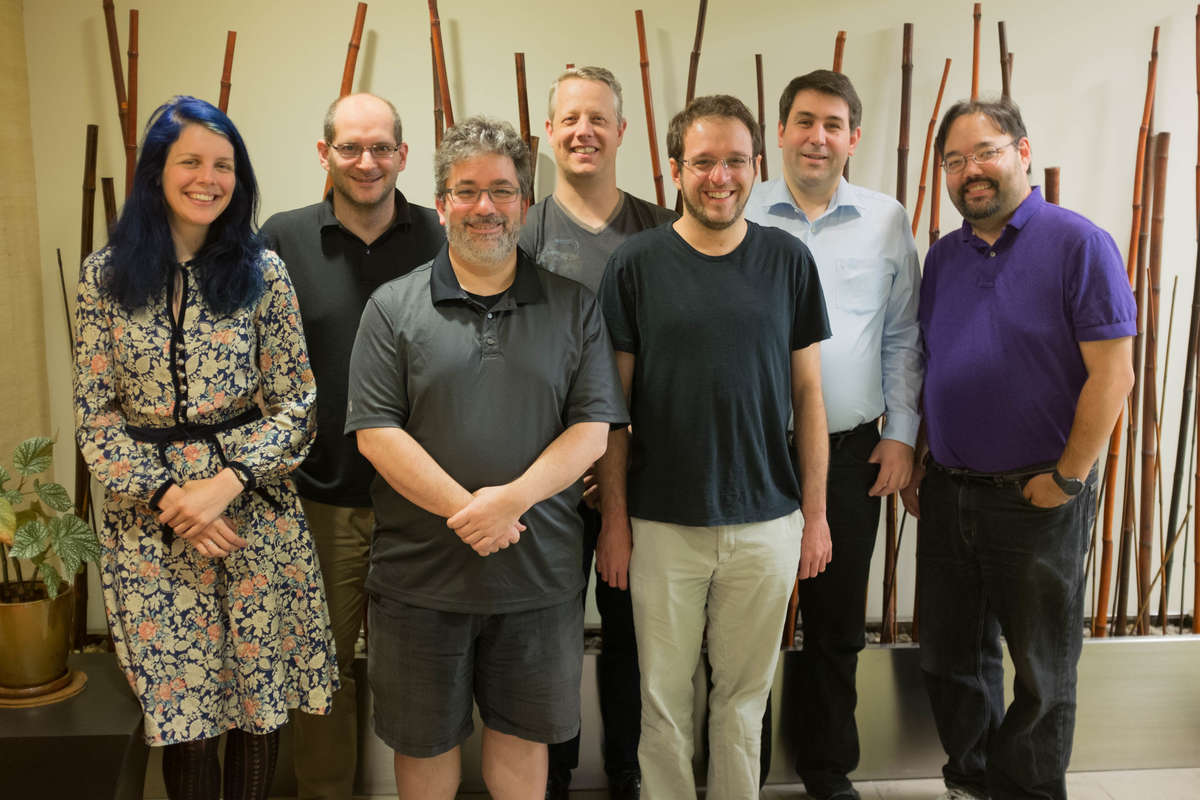
\includegraphics[scale=1.00]{images/2017-october-f2f}

\caption{Face-to-face meeting in New York (October 2017): Valerie Young,
Martin Michlmayr, Luca Filipozzi, Tim Potter, Jimmy Kaplowitz, Martin
Zobel-Helas and Michael Schultheiss (left to right)}

\end{figure*}

\chapter{Treasury Report}

This report uses a cash-based method of accounting, recording donations when
deposited (not when the check was written or received by us) and recording
expenses when sent or scheduled for payment (not when incurred).

\section{Income Statement}

This covers the Period January 1, 2017 -- December 31, 2017

\begin{verbatim}
TODO
\end{verbatim}

\section{Balance Sheet}

\begin{verbatim}
Balance Sheet as of December 31, 2017

TODO
\end{verbatim}

\chapter{Member Project Reports}

\section{New Associated Projects}

\section{Projects No Longer Associated with SPI}

\subsection{FreedomBox}

FreedomBox Foundation, the organizational headquarters of FreedomBox,
was recognized by the IRS as exempt from federal income tax under
Internal Revenue Code 501(c)(3).  Therefore, future donations will
be handled directly by the FreedomBox Foundation.

\section{Updates from Associated Projects}


\appendix
\chapter{About SPI}

SPI is a non-profit organization which was founded to help organizations
develop and distribute open hardware and software. We encourage programmers
to use the GNU General Public License or other licenses that allow free
redistribution and use of software, and hardware developers to distribute
documentation that will allow device drivers to be written for their product.

SPI was incorporated as a non-profit organization on June 16, 1997 in the state
of New York. Since then, it has become an umbrella organization for projects
from the community.

In 1999, the Internal Revenue Service (IRS) of the United States government
determined that under section 501 (a) of the Internal Revenue Code SPI
qualifies for 501 (c) (3) (non-profit organization) status under section 509
(a) (1) and 170 (b) (1) (A) (vi). This means that donations made to SPI and its
supported projects should be tax deductible for the American donor.

\end{document}
% Keep this at the bottom, thanks.
% Local Variables:
% TeX-master: "report"
% End:
